\chapter{Theoretical Background}\label{theoretical_background}

In this chapter, we will be covering the advanced theoretical background to fully understand the solved task of \gls{vrptw} using \gls{ai}.

\section{Reinforcement Learning}\label{rl}
    \gls{ml} can be divided with a little simplification into three categories; supervised learning, unsupervised learning, and reinforcement learning. Supervised learning is the most common where the model is learned from the provided labeled data. Unsupervised learning, on the other hand, is about finding a hidden patterns in a collection of data with no labels. Finally, reinforcement learning has no labeled data but learns by interacting with the environment and getting feedback in the form of rewards as shown in Figure \ref{fig:rl-loop}. 
    
    \begin{figure}[ht]
        \centering
        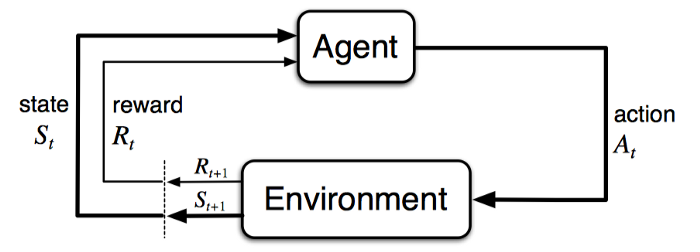
\includegraphics[width=0.75\textwidth]{resources/theoretical-background/rl-loop.png}
        \caption{Agent feedback loop\cite{rl-intro}}
        \label{fig:rl-loop}
    \end{figure}
    
    The Reinforcement Learning mimics the learning process of humans beings. By experiencing the world and accumulating knowledge, we are learning how to handle novel situations. \gls{rl} system consists of agent in observed state $s_t$, the agent interacts with the environment via its actions $a_t$ at discrete time steps $t$ and receives a reward $r_{t+1}$ for given action. The action moves the agent into a new state $s_{t+1}$. The goal of the agent is to learn a policy $\pi$ which chooses the action that maximizes the agent's rewards based on the environment \cite{rl-intro}. 
    
    %The policy is formally defined as a probability distribution of 
    \subsection{State and Action Value Functions}
        Transition to a new state gives us a reward and to maximize it, we need a way to quantify how good a state is. A state-value function $V_{\pi}(s)$ predicts a future reward for a given state when following the policy $\pi$ \cite{rl-intro}. 
    
        \begin{equation}
            V_{\pi}(s) = \mathop{\mathbb{E}}[G_t|S_t = s]
        \end{equation}
        \begin{equation}\label{discount-reward}
            G_t = \sum_{k=0}^{\infty} \gamma^k R_{t+k+1}
        \end{equation}
        The equation \ref{discount-reward} calculates $G_t$, all future rewards, sometimes called as $return$ \cite{rl-intro}. The $\gamma \in [0,1]$is a discount factor and penalizes the rewards in the future, incorporating the possible uncertainty and variance of the future rewards.
    
        We will also define action-value $Q_{\pi}(s, a)$ which is for a similar purpose as state-value function but predicts the reward for action and state following the policy $\pi$.
        \begin{equation}
            Q_{\pi}(s, a) = \mathop{\mathbb{E}}[G_t|S_t = s, A_t = a]
        \end{equation}
        
        The decomposition of state-value and action-value function replays on Bellman equations \cite{bellman-eq}. The decomposition of state-value function is
        \begin{equation}
            V_{\pi}(s) = \mathop{\mathbb{E}}[G_t|S_t = s]
        \end{equation}
        \begin{equation}
            V_{\pi}(s) = \mathop{\mathbb{E}}[R_{t+1} + \gamma R_{t+2} + \gamma^2 R_{t+3} + \cdots |S_t = s]
        \end{equation}
        \begin{equation}
            V_{\pi}(s) = \mathop{\mathbb{E}}[R_{t+1} + \gamma(R_{t+2} + \gamma R_{t+3} + \cdots) |S_t = s]
        \end{equation}
        \begin{equation}
            V_{\pi}(s) = \mathop{\mathbb{E}}[R_{t+1} + \gamma G_{t+1} |S_t = s]
        \end{equation}
        \begin{equation}
            V_{\pi}(s) = \mathop{\mathbb{E}}[R_{t+1} + \gamma V(S_{t+1}) |S_t = s]
        \end{equation}
        Similarly, this method is applicable to action-value function,
        \begin{equation}
            Q_{\pi}(s, a) = \mathop{\mathbb{E}}[R_{t+1} + \gamma V(S_{t+1}) |S_t = s, A_t = a]
        \end{equation}
        \begin{equation}
            Q_{\pi}(s, a) = \mathop{\mathbb{E}}[R_{t+1} + \gamma \mathop{\mathbb{E}}_{a \sim \pi} Q(S_{t+1}, a) |S_t = s, A_t = a]
        \end{equation}
    
        \subsection{Policy Gradients}
        Policy Gradient \cite{policy-gradient} is a method for solving the reinforcement learning problem and learning the policy that maximizes the rewards. We define a set of parameters $\theta$ that directly models the policy, $\pi_{\theta}(a|s)$.
    
        To optimize $\theta$ for the best reward, we define an objective function \cite{policy-gradient} as
        \begin{equation}
            J(\theta) = \sum_{s \in S} d_{\pi_{\theta}}(s)V_{\pi_{\theta}}(s)
        \end{equation}
        where $d_{\pi_{\theta}}(s)$ is stationary distribution of Markov chain for $\pi_{\theta}$, the probability of ending in a given state \cite{markov-bullshit}.
        \begin{equation}
            d_{\pi_{\theta}} = \lim_{t \longrightarrow \infty} P(S_t = s | s_0, \pi_{\theta})
        \end{equation}
        
        The objective function $J(\theta)$ optimizes the $\theta$ parameters via gradient ascent \cite{deep-learning}. 
        \begin{equation}
            \theta_{t+1} = \theta_{t} + \alpha \nabla J(\theta_{t})
        \end{equation}
        However, computing $\nabla J(\theta)$ is tricky because it depends on the action selection and the stationary distribution of states \cite{policy-weng}. Policy gradient can be simplified using Policy Gradient Theorem by Sutton et al. \cite{policy-gradient}.
        
        The proof of policy gradient theorem is quite long and complicated, but you may go through it in this article \cite{policy-weng} which is inspired by Sutton and Barto \cite{rl-intro}. Policy gradient is simplified to the form as
        \begin{equation}
            \nabla J(\theta) = \mathop{\mathbb{E}}[ \nabla \ln \pi (a|s, \theta) Q_{\theta}(s, a)]
        \end{equation}
    
        \subsection{REINFORCE}\label{reinforce}
        REINFORCE algorithm, proposed by Williams \cite{reinforce} in 1992, is a policy gradient method to update the policy parameter $\theta$.
        
        Let us define the additional terms required by the REINFORCE algorithm. We define a trajectory $\tau$ which is a sequence of states, actions, and rewards. Episode is a trajectory which ends at the terminal state $S_t$.
        \begin{equation}
            \tau = (S_0, A_0, R_0, S_1, A_1, R_1, \cdots)
        \end{equation}
        
        REINFORCE algorithm computes the policy gradient as follows
        \begin{equation}
            \nabla J(\theta) = \mathop{\mathbb{E}}[ G_{t} \nabla \ln \pi (A_t|S_t, \theta))]
        \end{equation}
        It is a simplification of a regular policy gradient because $Q_{\pi}(s, a) = \mathop{\mathbb{E}}[G_t|S_t = s, A_t = a]$ and in REINFORCE algorithm we rely on a full trajectory where we can estimate $G_t$ based on Monte-Carlo method which is describe in this article \cite{rl-intro}.
        
        \begin{algorithm}[H]
        \SetAlgoLined
        \KwResult{Updated $\theta$ that maximises reward}
         Initialize $theta$ at random\;
         Generate one episode $S_0, A_0, R_0, \cdots, S_T$\;
         \For{$t = 1, 2, \cdots, T$}{
          Estimate the the return $G_t$ since the time step t\;
          $\theta \gets \theta + \alpha \gamma^t G_t \nabla \ln \pi(A_t|S_t, \theta)$
         }
         \caption{REINFORCE algorithm}
        \end{algorithm}
        
        In the REINFORCE algorithm, the estimated gradient is highly effected by variance. A technique called baseline $b(S_t)$ is common to be used which subtracts a baseline from the estimated $G_t$ to reduce the variance \cite{baseline-artical}. The baseline function can be in many forms, but the most common one is to calculate the advantage function $A(s, a) = Q(s, a) - V(s)$ and use it to be subtracted from the gradient.

    \section{Attention}\label{attention}
    Attention mechanism was first proposed by Bahdanau et al.\cite{first-attention} in 2014 with a problem to help memorize long source sentences in neural machine translation. Not long after that, this concept gave birth to Transformers which dramatically improved many domains, especially Natural Language Processing and brought state-of-the-art results \cite{gpt-2}.
    
    \begin{figure}[ht]
        \centering
        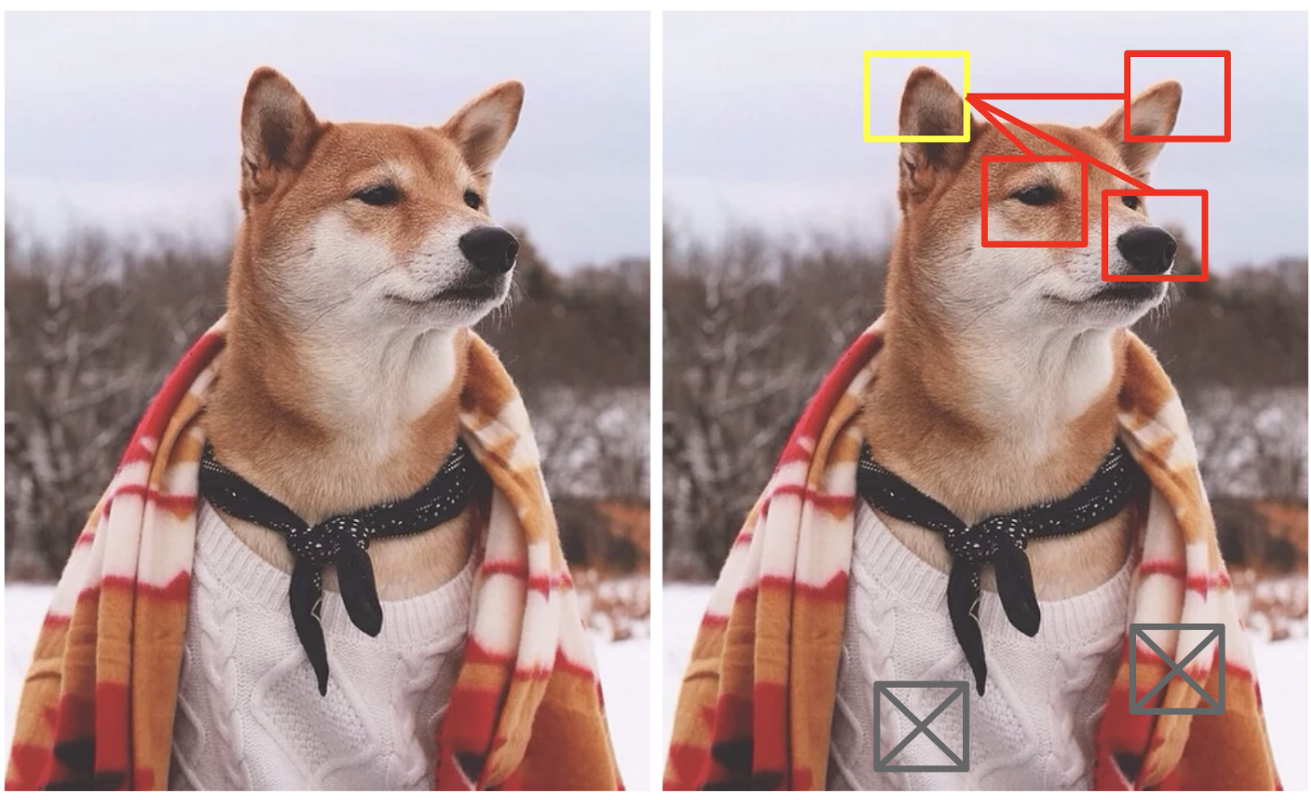
\includegraphics[width=0.5\textwidth]{resources/theoretical-background/shiba-attention.png}
        \caption{A Shiba Inu and what is caughting the network's attention \cite{attention-weng}, photo credit by @mensweardog.}
        \label{fig:shiba}
    \end{figure}
    
    For humans, visual attention is allowing us to focus on certain regions as visualized on Figure \ref{fig:shiba}. Attention mechanism decides on which part of the given source should pay attention to. 

        \subsection{Transformer}\label{transformer}
        The Transformer neural network architecture proposed by Vaswani et. al \cite{attention-is-all} was one of the major breakthroughs in the field of Natural Language processes (NLP). Transformer is getting rid of recurrence \cite{lstm} in favor of the attention mechanism which allows global dependencies between input and output. 
        %Additionally, they allows parallization 
        
        The Transformer architecture is based on encoder-decoder structure as shown on Figure \ref{fig:transformer}. Encoder maps the input sequence $x$ to continues representation $z$ which is taken by decoder and decodes it to output sequence $y$ one element at a time. The model is auto-regressive, it takes into account the previously generated output as additional input.
        
        \begin{figure}[ht]
            \centering
            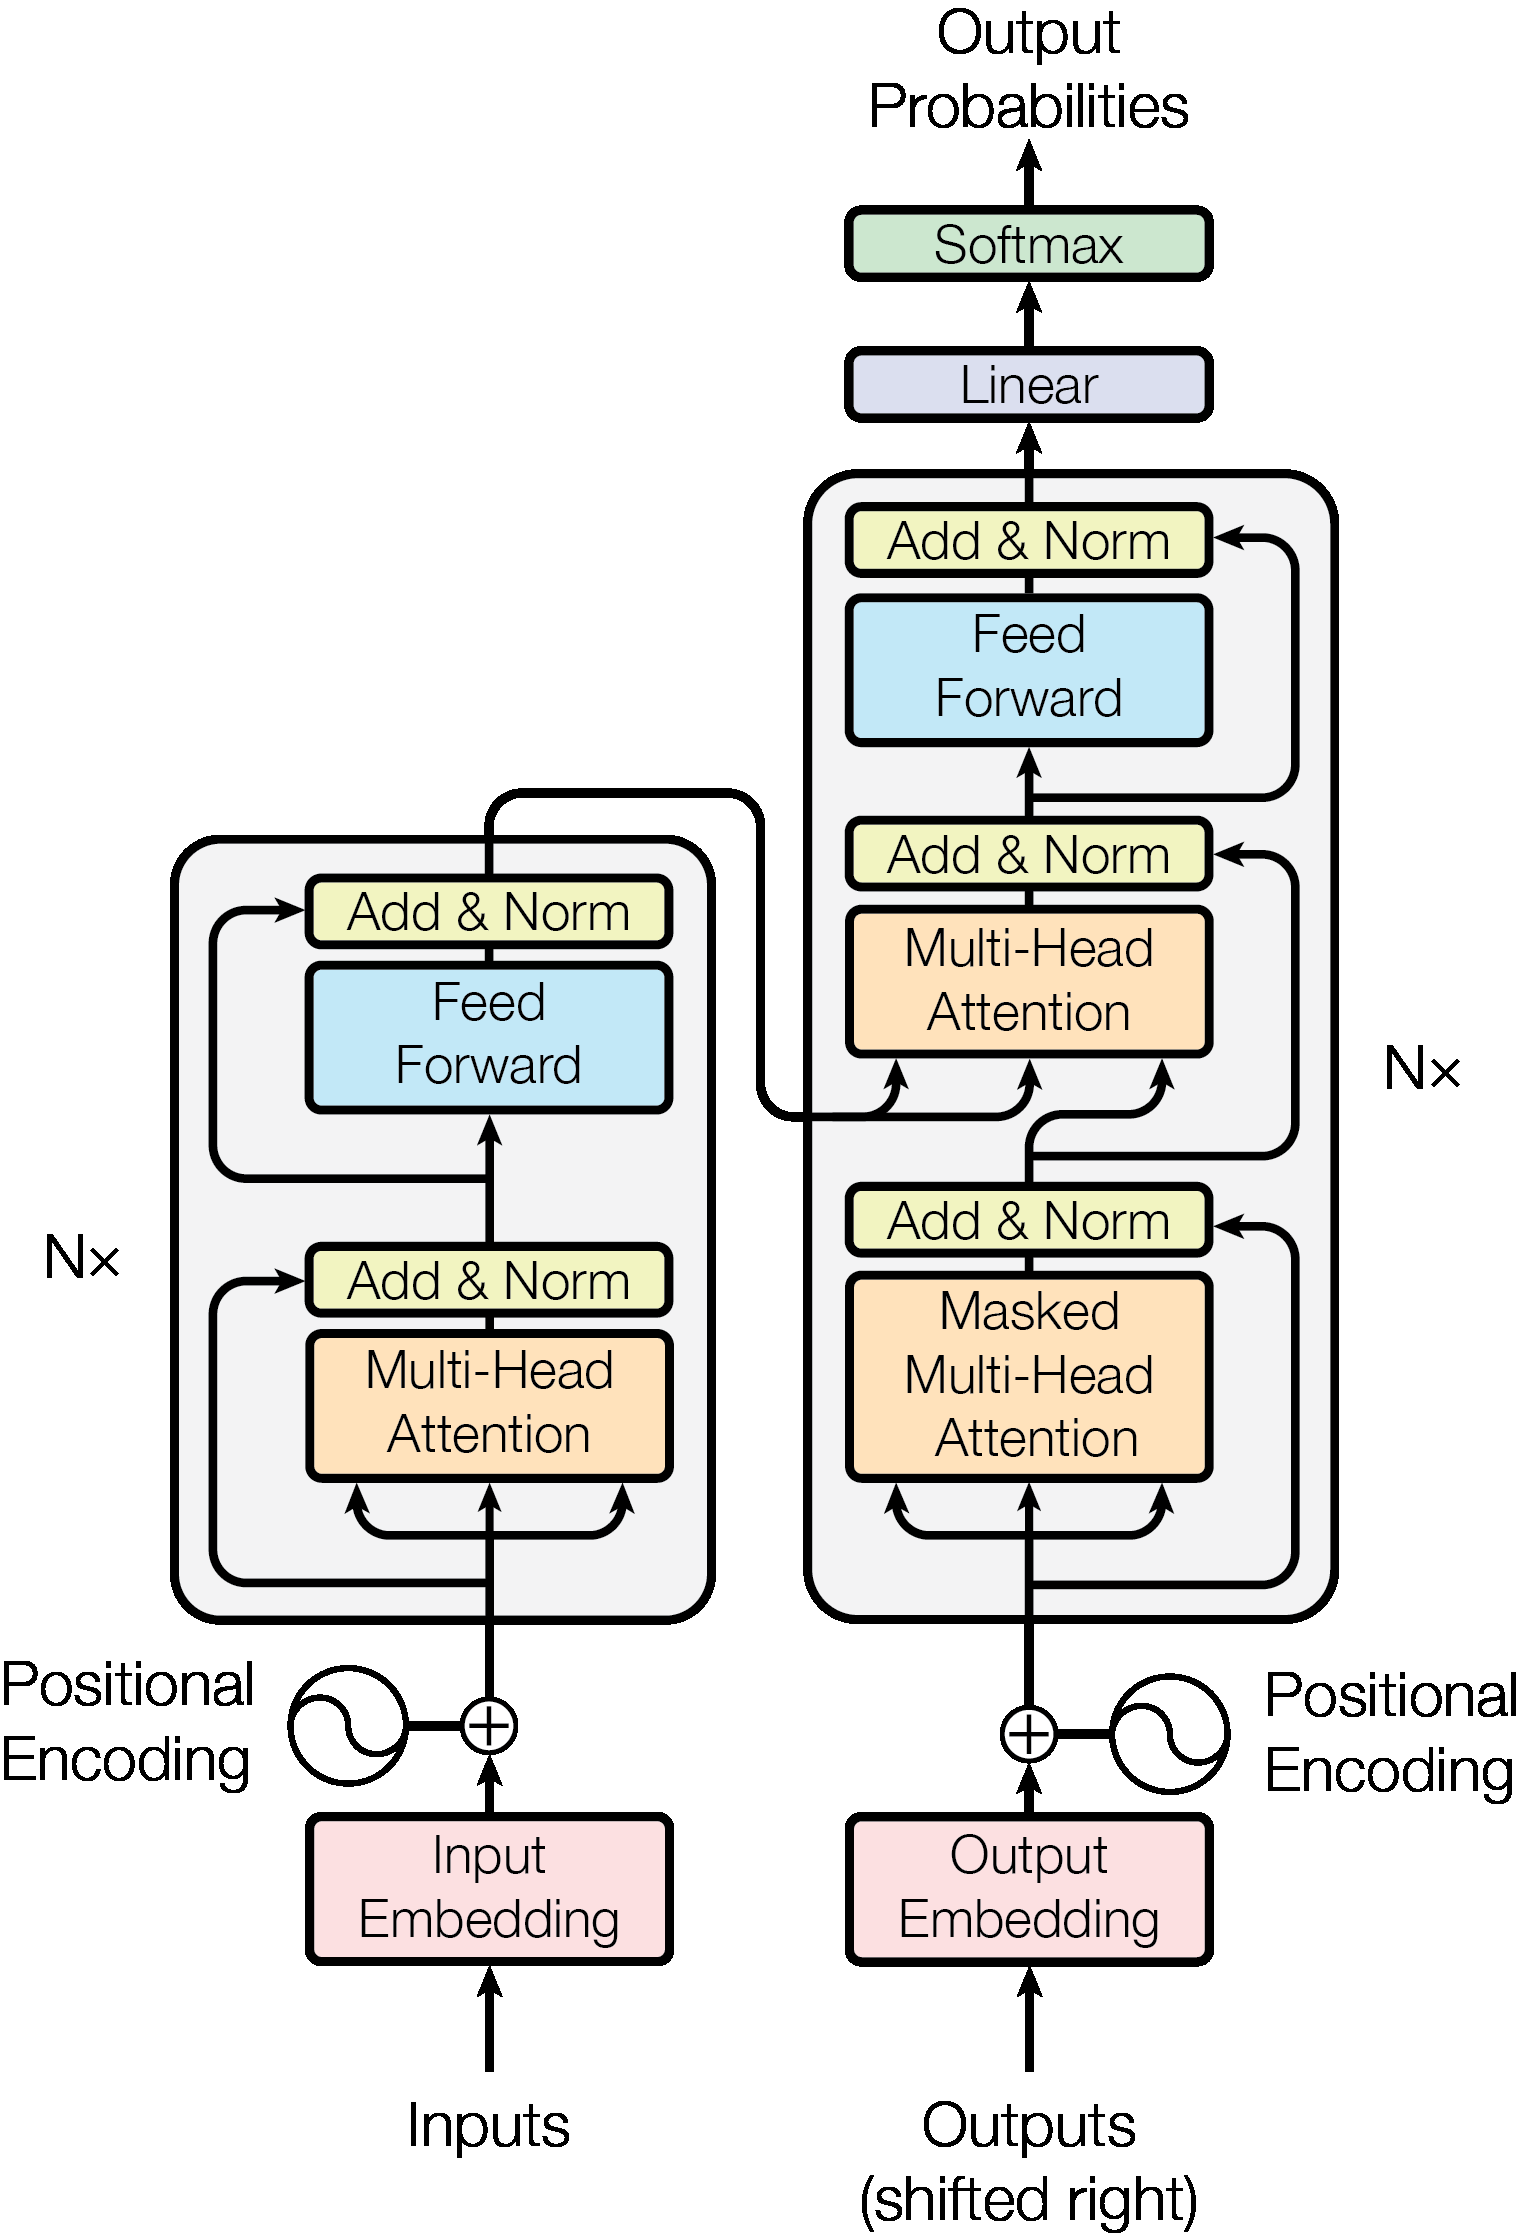
\includegraphics[width=0.5\textwidth]{resources/theoretical-background/transformer-arch.jpeg}
            \caption{The Transformer architecture, encoder on the left and decoder on the right \cite{attention-is-all}.}
            \label{fig:transformer}
        \end{figure}
        
            \subsubsection{Encoder}
            The encoder on Figure \ref{fig:transformer} has $N$ identical layers (Vaswani et al. set $N=6$ \cite{attention-is-all}). Each layer has two sublayers, the first is multi-head attention \ref{multi-head-attention}, and the second is a simple fully connected feed-forward network. Each of the sublayers has a residual connection \cite{residual-connection} that sums the input and output of the sublayer and normalize it \cite{normalization}. 
            
            \begin{equation}
                OutputSubLayer = Norm(x + SubLayer(x))
            \end{equation}
            
            The residual connections are similar to the skip connection which propagates input of the sublayer to the output which helps to avoid exploding or vanishing gradient.
            
            \subsubsection{Decoder}
            The decoder on Figure \ref{fig:transformer} is also built from $N$ identical layers and with similar sublayers as the encoder. The first sublayer is masked multi-head attention \ref{multi-head-attention} also with residual connection. The masking mechanism is only there to hide the future information because the Transformers are processing the input one by one. The next two sublayers of the decoder are same as the encoder with the only difference that multi-head attention \ref{multi-head-attention} receives part of the input from the encoder.
            
            \subsubsection{Multi-Head Attention}\label{multi-head-attention}
            The major component of Transformers is Multi-Head Attention (MHA). It runs the input through an attention mechanism $h$ times in parallel. The independent attention outputs are then concatenated and transformed into the expected dimension as shown in Figure \ref{fig:multi-head-attention} \cite{attention-weng}.
            
            \begin{figure}[ht]
                \centering
                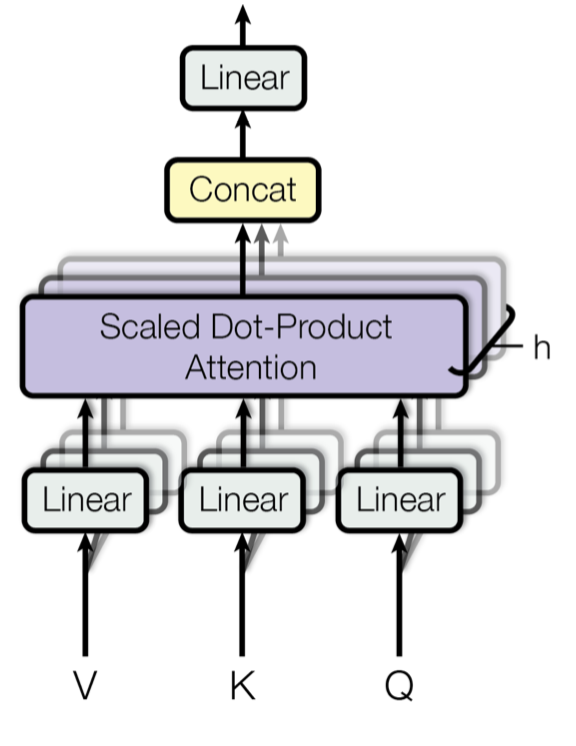
\includegraphics[width=0.5\textwidth]{resources/theoretical-background/multi-head-attention.png}
                \caption{Multi-Head Attention component \cite{attention-weng}}
                \label{fig:multi-head-attention}
            \end{figure}
            
            The Multi-Head Attention takes the embedded input and split the input copy to Key $K$, Value $V$ and Query $Q$. They all have the same dimension of input sequence length and embedded vector size $d_{\text{model}}$ (Vaswani et al. set $d_{\text{model}}=512$ \cite{attention-is-all}).
            
            The matrices $K$, $V$, and $Q$ get multiplied for each head $i \in (1, \cdots, $h$)$ by trainable parameters $W_i^K$, $W_i^V$, and $W_i^Q$, respectively. Then it performs scaled dot-product attention as shown in equations \ref{kvq} and \ref{scalled-dot-product}
            
            \begin{equation}\label{kvq}
                \text{head}_i = \text{ScaledDotAttention}(Q W_i^Q, K W_i^K, V W_i^Q)
            \end{equation}
            
            \begin{equation}\label{scalled-dot-product}
                \text{ScaledDotAttention}(Q, K, V) = \text{softmax}(\dfrac{Q K^T}{\sqrt{n}}) V
            \end{equation}
            
            According to the paper\cite{attention-is-all}, the scaled dot product attention allows the model to jointly attend to information from different representation subspaces at different positions.
            
            Finally, we concatenate all head outputs $head_i$ for $i \in (1, \cdots, $h$)$ from scaled dot product attention and perform linear transformation by trainable parameter $W_0$ of \gls{mha}.
            \begin{equation}
                \text{MHA}(Q, K, V) = \text{Concat}(\text{head}_1, \cdots, \text{head}_h)W_0
            \end{equation}
            
        \subsection{Graph Attention Network}\label{graph-attention-network}
        To understand the model used for solving \gls{vrptw} we need a basic understanding of \gls{gat}, first proposed by Veličković et al. \cite{gat} in 2017.
        
        It is a neural network architecture capable of operating on graph-structured data. \gls{gat} extend the work on Graph Convolution Networks \cite{gcn} which has a problem with generalizability because they are structure-dependent \cite{dgl-gat}. \gls{gat} address the shortcoming of \gls{gcn} by leveraging masked self-attentional layers \ref{attention}.
        
        \gls{gat} is a single layer (possibly can be stacked) which takes a set of nodes features $h = \{h_0, h_1, \cdots, h_N\}, h_i \in \mathbb{R}^F$ where N is the number of nodes and $F$ is the number of features for a node. The \gls{gat} layer assigning different importance to each node through the attention coefficients.
        
        \begin{equation}\label{edge-attention}
            e^l_{ij} = a^l(W^l h_i^l, W^l h_j^l)
        \end{equation}
        
        The equation \ref{edge-attention} is a linear transformation of node features and weight matrix $W^l$ which is used for calculating the attention coefficients via learnable parameter $a^l$. It is gathering information about the importance of node j’s features to node i.
        
        \begin{equation}\label{neighbout-attention}
            \alpha_{ij}^l = \text{softmax}_j(e^l_{ij}) = \dfrac{exp(e^l_{ij})}{\sum_{k \in N_i} exp(e^l_{ik}}
        \end{equation}
        
        The graph structural data are represented in attention via equation \ref{neighbout-attention} which is computed only for all neighbour nodes $N_i$ of node i. The softmax function is used to make the attention scores comparable across different nodes. 
        
        \begin{equation}\label{next-layer}
            h_{i}^{l+1} = \sigma(\sum_{j \in N_i} \alpha_{ij}^l W^l h_i^l)
        \end{equation}
        
        The equation \ref{next-layer} is aggregating together all attention embeddings of all neighbour nodes. If we perform multi-head attention on the final layer of \gls{gat} then computation of the final high level feature embedding is as follows
        
        \begin{equation}
            h_{i}^{l+1} = \sigma(\dfrac{1}{K} \sum_{k = 1}^K \sum_{j \in N_i} \alpha_{ij}^l W^k h_i^l)
        \end{equation}
        
        The aggregation process of a multi-head graph attentional layer for a given node is illustrated on Figure \ref{fig:gat-diagram}.
        
        \begin{figure}[ht]
            \centering
            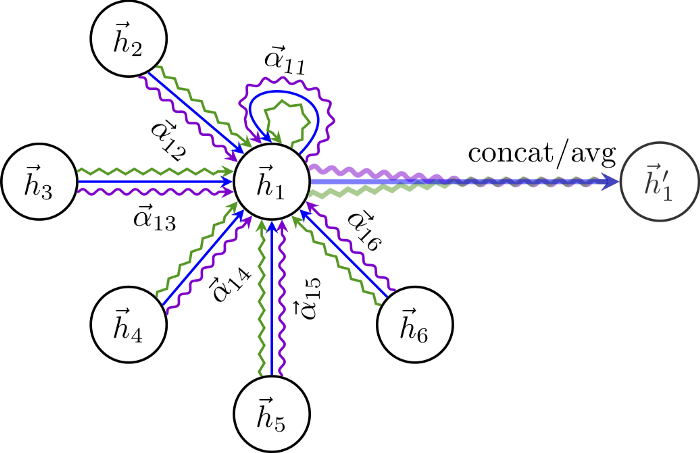
\includegraphics[width=0.75\textwidth]{resources/theoretical-background/gat-diagram.png}
            \caption{Multi-head attention with $K = 3$ heads \cite{gat}.}
            \label{fig:gat-diagram}
        \end{figure}
    
    

